\usepackage[english]{babel}
\usepackage{fancyhdr}


% -----------------------------------------------------------------------------
% command.tex
% This file contains the various package imports, environment declarations,
% and other miscellaneous commands.
% -----------------------------------------------------------------------------

% \usepackage{pkgloader}            % Use this to resolve package dependencies

\usepackage{algorithmicx}
\usepackage{amsmath, amsfonts, amscd, amssymb}
\usepackage{appendix}
\usepackage{array}
% \usepackage{bbm}
\usepackage{bigstrut}
\usepackage{blkarray}
\usepackage{color}
\usepackage{colortbl}
\usepackage{epsfig}
\usepackage{float}
\usepackage{framed}
\usepackage{gensymb}
\usepackage{graphicx}
\usepackage{hyperref}
\usepackage{import}
\usepackage{listings}
\usepackage{mathrsfs}
\usepackage{mathtools}
\usepackage{makeidx}
\usepackage{multicol}
\usepackage{multirow}
\usepackage{paralist}
\usepackage{relsize}
\usepackage{subcaption}
\usepackage{textcomp}
\usepackage{verbatim}
\usepackage{tikz}
\usepackage{xparse}
\usepackage{xcolor}
\usepackage{url}

\usepackage[plain]{algorithm}
\usepackage[noend]{algpseudocode}
% \usepackage[style=alphabetic,refsection=chapter,backref=true,backend=bibtex]{biblatex}
\usepackage[customcolors]{hf-tikz}
\usepackage[framemethod=tikz]{mdframed}

% \usepackage{caption}
% \usepackage{subcaption}
% \usepackage{textcomp}
%\input{macros}

% \LoadPackagesNow                  % Use this to resolve package dependencies

% Tikzpicture tools
\usetikzlibrary{arrows, automata, backgrounds, calendar, chains, decorations,
    matrix, mindmap, patterns, petri, positioning, shadows, shapes.geometric,
    trees, shapes, decorations.pathreplacing}
\usetikzlibrary{circuits.ee.IEC}

% Document settings ===========================================================

% Colors
\definecolor{red}{cmyk}{0, 1.00, 0.62,0}
\definecolor{blue}{cmyk}{1.00, .34, .0 .02 }    % blue
\definecolor{green}{cmyk}{0.7, 0, 1.0, 0.09 }   % greenish
\definecolor{yellow}{cmyk}{0, 0.16, 1.0, 0}     % yellow
\definecolor{gray}{cmyk}{0, 0, 0, 0.65}         % gray
\definecolor{purple}{cmyk}{.333, .867, 0, .059}

\hfsetfillcolor{red!02}
\hfsetbordercolor{red}

% Set lengths that are pleasing for screen display.
\setlength{\paperheight}{11in}
\setlength{\paperwidth}{8.5in}

% Set paragraph skips and line spacing
\linespread{1.05}
\setlength{\parskip} {2pt plus1pt minus1pt}

\makeatletter

% Make all floats centered
\g@addto@macro\@floatboxreset\centering

% Reset footnote counter every chapter
\@addtoreset{footnote}{chapter}
\makeatother

\floatstyle{ruled}
\restylefloat{algorithm}

\makeatletter
\Hy@AtBeginDocument{
    \def\@pdfborder{0 0 1}
    \def\@pdfborderstyle{/S/U/W 1}
}
\makeatother

% Make margins the same on both sides (independent of odd or even page)
 \newlength{\marg}
 \setlength{\marg}{1.23in} %% Set the desired margin length here.
 \usepackage{marginnote}
 %\usepackage[inner=1.0\marg,top=\marg,outer=1.0\marg, bottom=\marg, marginparsep = 0.25em, marginparwidth = .7\marg]{geometry}


% Lab Commands ================================================================




\newcommand{\objective}[1]{{\bf Lab Objective: } \emph{#1} \bigskip}

%% Full line comments in the Algorithmic environment.
\algnewcommand{\LineComment}[1]{\State \(\triangleright\) #1}


% Misc. Environments ==========================================================


%\newcounter{problemnum}[chapter]
%\newenvironment{problem}{\begin{mdframed}[style=problem]\begin{problemnum}}{\end{problemnum}\end{mdframed}}
%\newtheorem{problemnum}{Problem}
%
%\newenvironment{problem*}{\begin{mdframed}[style=problem]\begin{problemnum*}}{\end{problemnum*}\end{mdframed}}
%\newtheorem{problemnum*}[problemnum]{*Problem}


% Colors ======================================================================


\colorlet{shadecolor}{blue!10}
%\definecolor{shadecolor}{RGB}{186, 207, 188}
\colorlet{warning}{red!20!}       %{RGB}{255, 188, 163}
\colorlet{warnline}{red}          %{RGB}{255, 15, 15}
\colorlet{information}{green!20}
\colorlet{infoline}{green}
%\definecolor{information}{RGB}{235, 255, 223}
%\definecolor{infoline}{RGB}{69, 163, 11}
\colorlet{codebase}{yellow!30!}
\colorlet{codekeyword}{blue}
\colorlet{codecomment}{green}
\colorlet{codestring}{red}


% Frame environments ==========================================================


\mdfdefinestyle{problem}{backgroundcolor=shadecolor,
                        skipabove=10pt,
                        skipbelow=10pt
                        leftmargin=20pt,
                        rightmargin=20pt,
                        innertopmargin=10pt,
                        innerbottommargin=10pt,
                        innerleftmargin=10pt,
                        middlelinewidth=0pt,
                        everyline=true,
                        linecolor=blue,
                        linewidth=2pt}

\newmdenv[
  %roundcorner=10pt,
  skipabove=10pt
  skipbelow=10pt
  leftmargin=20pt,
  rightmargin=20pt,
  backgroundcolor=warning,
  innertopmargin=10pt,
  innerbottommargin=10pt,
  innerleftmargin=10pt,
  middlelinewidth=0pt,
  everyline=true,
  linecolor=warnline,
  linewidth=2pt,
  font=\normalfont\normalsize,
  frametitlefont=\large\bfseries,
  frametitleaboveskip=1em,
  frametitlerule=true,
  frametitle={\sc Achtung!}
]{warn}


\newmdenv[
  %roundcorner=10pt,
  skipabove=10pt,
  skipbelow=10pt,
  leftmargin=20pt,
  rightmargin=20pt,
  backgroundcolor=information,
  outerlinewidth=0pt,
  outerlinecolor=infoline,
  innertopmargin=10pt,
  innerbottommargin=10pt,
  innerleftmargin=10pt,
  middlelinewidth=0pt,
  everyline=true,
  linecolor=infoline,
  linewidth=2pt,
  font=\normalfont\normalsize,
  frametitlefont=\large\bfseries,
  frametitleaboveskip=1em,
  frametitlerule=true,
  frametitle={\sc Note}
]{info}


%% Listings Environments ======================================================


% Default Environment
\lstset{
  language=Python,
  backgroundcolor=\color{codebase},   %\color[RGB]{250, 245, 182},
  tabsize=4,
  basewidth=.5em,
  rulecolor=\color{yellow},           %\color{black},
  basicstyle=\normalsize\ttfamily,    % code text size
  upquote=true,
  columns=fixed,
  extendedchars=true,
  breaklines=true,
  prebreak = \raisebox{0ex}[0ex][0ex]{\ensuremath{\hookleftarrow}},
  frame=lrtb,
  xleftmargin=5pt,
  xrightmargin=5pt,
  framesep=4pt,
  framerule=2pt,
  showtabs=false,
  showspaces=false,
  showstringspaces=false,
  morestring=[s]{"""}{"""},
  morestring=[s]{'''}{'''},
  keywordstyle=\color{codekeyword},   %\color[RGB]{42, 161, 152},
  commentstyle=\color{codecomment},   %\color[RGB]{108, 153, 8},
  stringstyle=\color{codestring},     %\color[RGB]{189, 78, 98},
  title=\lstname,
  captionpos=b,
  abovecaptionskip=-5pt,
  belowcaptionskip=-5pt,
  moredelim=[is][\color{black}]{<<}{>>},
  moredelim=[is][\color{red}]{<r<}{>r>},
  moredelim=[is][\color{blue}]{<b<}{>b>},
  moredelim=[is][\color{green}]{<g<}{>g>},
  moredelim=[is][\color{purple}]{<p<}{>p>},
  morekeywords={assert, bytes, self, super, with, as, yield, True, False, None, NotImplemented, BaseException, Exception, AssertionError, AttributeError, ImportError, IndexError, KeyError, KeyboardInterrupt, MemoryError, NameError, NotImplementedError, OSError, OverflowError, RecursionError, RuntimeError, StopIteration, SyntaxError, IndentationError, TabError, StandardError, SystemError, SystemExit, TypeError, ValueError, ZeroDivisionError, IOError, Warning, RuntimeWarning, FileExistsError, FileNotFoundError,
    SELECT, FROM, AS, INNER, JOIN, LEFT, OUTER,
    CROSS, ON, WHERE, CASE, IF,
    MIN, MAX, SUM, AVG, COUNT,
    TEXT, REAL
  },
  deletekeywords={compile, format}
}

% \surroundwithmdframed[
%         hidealllines=true,
%         backgroundcolor=codebase,
%         innerleftmargin=-5pt,
%         innertopmargin=-1pt,
%         innerrightmargin=0pt,
%         innerbottommargin=-5pt]{lstlisting}

% Including source code from a file on disk
\lstdefinestyle{FromFile}{language=Python,
                          frame=single,
                          numbers=left,
                          numberstyle=\tiny,
                          stepnumber=2,
                          numbersep=7pt,
                          numberfirstline=true,
                          abovecaptionskip=2pt,
                          belowcaptionskip=2pt
                          }

% Shell I/O.  Avoids syntax highlighting
\lstdefinestyle{ShellOutput}{language=}
\lstdefinestyle{ShellInput}{language=}

%% Deprecated Environments (Replaced by Algorithmic package)
\lstdefinestyle{pseudo}{basicstyle=\rmfamily,
                        upquote=true,
                        keywordstyle=\color{black}\bfseries,
                        commentstyle=\color[rgb]{0.133,0.545,0.133},
                        stringstyle=\color[rgb]{0.627,0.126,0.941},
                        }

\newcommand{\pseudoli}[1]{\lstinline[style=pseudo]!#1!}
\newcommand{\li}[1]{\lstinline[prebreak=]!#1!}
\newcommand{\lif}[1]{\lstinline[basicstyle=\footnotesize\ttfamily,language=Python,prebreak=]!#1!} % for inline code in footnotes.
\newcommand{\lsql}[1]{\lstinline[language=SQL,prebreak=,
                                morekeywords={TEXT, REAL, IF}]!#1!}


% Special Math Characters =====================================================


\def\0{\mathbf{0}}
%\def\0{0}
\def\a{\mathbf{a}}
%\def\b{\mathbf{b}}
%\renewcommand{\b}{b}
%\def\b{b}
\def\c{\mathbf{c}}
\def\e{\mathbf{e}}
\def\f{\mathbf{f}}
\def\g{\mathbf{g}}
\def\p{\mathbf{p}}
\def\q{\mathbf{q}}
\def\u{\mathbf{u}}
\def\v{\mathbf{v}}
\def\w{\mathbf{w}}
\def\x{\mathbf{x}}
\def\y{\mathbf{y}}
\def\z{\mathbf{z}}
\def\subspace{\lhd}

\def\CalL{\mathcal{L}}
\def\CalO{\mathcal{O}}
\def\CalV{\mathcal{V}}
\def\CalU{\mathcal{U}}
\def\bU{{\bar{u}}}
\def\R{\Re e}
\def\I{\Im m}
\def\M{M_n}

\def\lvl#1{\multicolumn{1}{|c}{#1}} % Left  Vertical Line in array cell.
\def\rvl#1{\multicolumn{1}{c|}{#1}} % Right Vertical Line in array cell.

% Various other shortcuts =====================================================

\renewcommand{\epsilon}{\varepsilon}                    % curly epsilon
\newcommand{\argmax}{\mbox{argmax}}
\newcommand{\indicator}{\boldsymbol{1}}
% \newcommand{\indicator}{\mathbbm{1}} % characteristic (indicator) function
% ^Travis hates this, but it would be nice to have bbm instead.
\providecommand{\abs}[1]{\left\lvert#1\right\rvert}
\providecommand{\norm}[1]{\left\lVert#1\right\rVert}
\providecommand{\set}[1]{\lbrace#1\rbrace}
\providecommand{\setconstruct}[2]{\lbrace#1:#2\rbrace}
%\providecommand{\Res}[1]{\underset{#1}{Res}}            % Residue
\newcommand{\trp}{^{\mathsf T}}                         % matrix transpose
\newcommand{\hrm}{^{\mathsf H}}                         % hermitian conjugate

\newcommand{\ipt}[2]{\langle #1,#2 \rangle}
\newcommand{\ip}{\int_{-\infty}^{+\infty}}

\renewcommand{\ker}[1]{\mathcal{N}(#1)}
\newcommand{\ran}[1]{\mathcal{R}(#1)}

% For making block arrays with correct bracket sizes
\newcommand\topstrut[1][0.8ex]{\setlength\bigstrutjot{#1}{\bigstrut[t]}}
\newcommand\botstrut[1][0.6ex]{\setlength\bigstrutjot{#1}{\bigstrut[b]}}

% These commands are specifically for use in the pseudocode environment.
% Load the xparse package to use these commands
\NewDocumentCommand\allocate{m+g}{                      % Empty array
  \IfNoValueTF{#2}
    {\mathrm{empty}(#1)}                                % 1 dimension
    {\mathrm{empty}(#1, #2)}                            % 2 dimensions
}

\NewDocumentCommand\zeros{m+g}{                         % Zero array
  \IfNoValueTF{#2}
    {\mathrm{zeros}(#1)}
    {\mathrm{zeros}(#1, #2)}%
}

\newcommand{\Id}[1]{\mathrm{Id}(#1)}                    % Identity array
\newcommand{\makecopy}[1]{\mathrm{copy}(#1)}            % Copy an array
\newcommand{\shape}[1]{\mathrm{shape}(#1)}
\newcommand{\size}[1]{\mathrm{size}(#1)}


% Math Operators ==============================================================

% Many of these are for use in the pseudocode environments.
\DeclareMathOperator{\sign}{sign}
\DeclareMathOperator{\sech}{sech}
\DeclareMathOperator{\Out}{Out}                         % Used in PageRank lab
\DeclareMathOperator{\In}{In}                           % Used in PageRank lab
\DeclareMathOperator\erf{erf}



\newcommand{\contributor}[2]{\noindent\vtop{\hsize14pc#1\\\itshape#2}\par}

\newenvironment{contributors}{{List of Contributors}%
%\addcontentsline{toc}{chapter}{List of Contributors}%
             \thispagestyle{plain}\begin{multicols}{2}\parindent0pt%
\parskip6pt plus2pt minus1pt%
\widowpenalty10000\clubpenalty10000}
               {\end{multicols}   
               This project is funded in part by the National Science Foundation, grant no. TUES Phase II DUE-1323785.            
               \clearpage}





\usepackage{algorithm}%,algpseudocode}
\usepackage{mdframed}
\usepackage{longtable}


\cellcolor{red}

%\newcommand{\cr}[1]{\mathbf{#1}} % change to \mathbb

\newcommand{\rc}{\cellcolor{red}} % change cell color red in table
\newcommand{\hi}{\cellcolor{red}} % change cell color red in table

%\newtheorem{example}{Example}%[section]
\newtheorem{ICE}{ICE}%[section]
%\newtheorem{problem}{Problem}%[section]
%\newtheorem{solution}{Solution}%[section]

%\def\input@path{{/figures/}}
%\def\input@path{{/path/to/folder/}{/path/to/other/folder/}}

\newcounter{algsubstate}
\renewcommand{\thealgsubstate}{\alph{algsubstate}}
\newenvironment{algsubstates}
  {\setcounter{algsubstate}{0}%
   \renewcommand{\State}{%
     \stepcounter{algsubstate}%
     \Statex {\footnotesize\thealgsubstate:}\space}}
  {}


%\numberwithin{equation}{section}

\graphicspath{{figures/}{optimization/figures/figures-static/}}
\usepackage{wasysym}
\newsavebox\CBox
\newcommand\hcancel[2][0.5pt]{%
  \ifmmode\sbox\CBox{$#2$}\else\sbox\CBox{#2}\fi%
  \makebox[0pt][l]{\usebox\CBox}%  
  \rule[0.5\ht\CBox-#1/2]{\wd\CBox}{#1}}

\usepackage[cc]{titlepic}
\usepackage{xcolor}
\colorlet{notgreen}{blue!50!yellow}
\newcommand{\tblue}[1]{{\color{blue} #1}}
\newcommand{\tred}[1]{{\color{red} #1}}
\newcommand{\tgreen}[1]{{\color{notgreen} #1}}

\newcommand{\code}[1]{\texttt{ #1}}
\newcommand{\complexity}[1]{{\color{red} \textit{#1}}}
\newcommand{\nphard}{\complexity{NP-Hard}}
\newcommand{\npcomplete}{\complexity{NP-Complete}}
\newcommand{\polynomial}{{\color{ansi-green} \textit{Polynomial time (P)}}}
\newcommand{\true}{\tgreen{\texttt{ true }}}
\newcommand{\false}{\tred{\texttt{ false }}}

\usepackage{scalerel}
\newcommand{\julia}{\raisebox{-.2\height}{
\includegraphics[scale = 0.07]{julia-logo}}  }
\newcommand{\jupyter}{\raisebox{-.2\height}{
\includegraphics[scale = 0.09]{jupyter-logo}}  }
\newcommand{\jump}{\raisebox{-.2\height}{
\includegraphics[scale = 0.08]{jump-logo}}  }
\newcommand{\gurobi}{\raisebox{-.2\height}{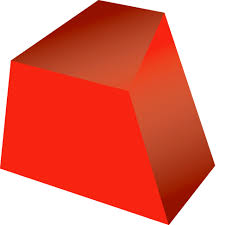
\includegraphics[scale = 0.06]{gurobi-logo}}Gurobi  }
\newcommand{\coin}{\raisebox{-.2\height}{
\includegraphics[scale = 0.2]{coin-or-logo}}  }
\newcommand{\ipopt}{\raisebox{-.2\height}{\texttt{Ipopt}}}


\usepackage{subcaption}

\def \PP{ {\mathcal{P}}}
\def \NN{ {\mathcal{N}}}
\def \II{ {\mathcal{I}}}
\def \ZZ{ {\mathcal{Z}}}
\def \SS{ {\mathcal{S}}}
\def \FF{ {\mathcal{F}}}
\def \CC{ {\mathcal{C}}}
\def \nn{ {\mathbb{N}}}
\def \R{ {\mathbb{R}}}
\def \Z{ {\mathbb{Z}}}
\def \Q{ {\mathbb{Q}}}
\def \cc{ {\mathbb{C}}}

\DeclareMathOperator{\dom}{dom}
\DeclareMathOperator{\cl}{cl}
\DeclareMathOperator{\intr}{intr}

\def \rank{\textup{rank}}
\def \size{\textup{size}}
%\def \dist{\textup{dist}}
\def \sign{\textup{sign}}
\def \deg{\textup{deg}}
\def \conv{\textup{conv}}
\def \cone{ {\textup{cone}}}
\def \supp{\textup{supp}}
\def \int{ {\textup{int}}}
\def \rc{\textup{rec.cone}}
\def \ri{\textup{rel.int}}
\def \rb{ {\textup{rel.bd}}}
\def \bd{ {\textup{bd}}}
\def \ls{\textup{lin.space}}
\def \tq{{\,:\,}}
\def \aff{{\textup{aff}}}
\def \one{\mathbb{1}}
\def \st{ \text{ s.t. }}

\def \BQP{\mathrm{BQP}}
\def \xLP{x^{\mathrm{LP}}}
\DeclareMathOperator    \argmin         {arg\,min}
%\DeclareMathOperator    \argmax         {arg\,max}


%\newcounter{example}
\newcounter{general}

  % Test Environment
  \newcounter{exo}
\makeatletter
\newenvironment{exo}[1]%
{\refstepcounter{exo}%
\protected@edef\@currentlabelname{Exercise \theexo: #1}% addition here
\vspace{0.5cm}\noindent
{\large\bfseries{Exercise \theexo~: #1} \par}
{\par\vspace{0.5cm}}}
\makeatother

\newcounter{codeCell}
\makeatletter
\newenvironment{codeCell}%
{\refstepcounter{codeCell}%
\protected@edef\@currentlabelname{Code}% addition here
{}
%{\large\bfseries{Exercise \theexo~: #1} \par}
{}}
\makeatother

% General environment
\newenvironment{general}[2]
  {\par\medskip
   %\refstepcounter{exo}%
  \protected@edef\@currentlabelname{#1}
   \begin{framed}
   \begingroup\color{black}%
   \textbf{#1: }\ignorespaces
   \par #2
   \par}
 {\endgroup\end{framed}
  \medskip}
  

 % Example Environment
  \newenvironment{optexample}
  {\par\medskip
  \refstepcounter{exo}%
  \protected@edef\@currentlabelname{Example \theexo}
   \begin{framed}
   \begingroup\color{blue}%
   \textbf{Example \theexo: }\ignorespaces}
 {\endgroup\end{framed}
  \medskip}
  
  
  % Example with code Environment
   \newenvironment{examplewithcode}[2]
  {\par\medskip
   \refstepcounter{exo}%
  \protected@edef\@currentlabelname{Example \theexo}
  \begin{center}
 \rule{\textwidth}{0.4pt}\\
 \vspace{-0.2cm}
 \rule{\textwidth}{0.4pt}
 \end{center}
   %\begin{framed}
   \begingroup\color{black}%
   \textbf{Example: #1}
   \hfill \protect\href{#2}{Gurobipy}% code link somehow
    \ignorespaces
    \par}
 { \endgroup
 %\end{framed}
   \begin{center}
 \rule{\textwidth}{1.8pt}
 \end{center}
  \medskip}
  
    % Example with all code Environment
   \newenvironment{examplewithallcode}[4]
  {\par\medskip
   \refstepcounter{exo}%
  \protected@edef\@currentlabelname{Example \theexo}
   \begin{framed}
   \begingroup\color{black}%
   \textbf{Example: #1}
   \hfill \protect\href{#2}{ \ Excel \ }\protect\href{#3}{ \ PuLP \ }\protect\href{#4}{\ Gurobipy \ }% code link somehow
    \ignorespaces
    \par}
 { \endgroup
 \end{framed}
  \medskip}
  
    % Example without code Environment
   \newenvironment{examplewithoutcode}[2]
  {\par\medskip
   \refstepcounter{exo}%
  \protected@edef\@currentlabelname{Example \theexo}
   \begin{framed}
   \begingroup\color{black}%
   \textbf{Example: #1}
    \ignorespaces
    \par}
 { \endgroup
 \end{framed}
  \medskip}
  

\newcommand{\floor}[1]{\lfloor #1 \rfloor}
\newcommand{\ceil}[1]{\lceil #1 \rceil}


\newcommand{\mathup}[1]{#1}
\newcommand{\NP}{\text{NP}}
\newcommand{\coNP}{\text{coNP}}




    \usepackage[T1]{fontenc}
    % Nicer default font (+ math font) than Computer Modern for most use cases
    %\usepackage{mathpazo}

    % Basic figure setup, for now with no caption control since it's done
    % automatically by Pandoc (which extracts ![](path) syntax from Markdown).
    \usepackage{graphicx}
    % We will generate all images so they have a width \maxwidth. This means
    % that they will get their normal width if they fit onto the page, but
    % are scaled down if they would overflow the margins.
    \makeatletter
    \def\maxwidth{\ifdim\Gin@nat@width>\linewidth\linewidth
    \else\Gin@nat@width\fi}
    \makeatother
    %\let\Oldincludegraphics\includegraphics
    % Set max figure width to be 80% of text width, for now hardcoded.
   % \renewcommand{\includegraphics}[1]{\Oldincludegraphics[width=.8\maxwidth]{#1}}
    % Ensure that by default, figures have no caption (until we provide a
    % proper Figure object with a Caption API and a way to capture that
    % in the conversion process - todo).
    \usepackage{caption}
   % \DeclareCaptionLabelFormat{nolabel}{}
    %\captionsetup{labelformat=nolabel}

    \usepackage{adjustbox} % Used to constrain images to a maximum size 
    %\usepackage[table]{xcolor} % Allow colors to be defined
    %\usepackage{enumerate} % Needed for markdown enumerations to work
    %\usepackage{geometry} % Used to adjust the document margins
    %\usepackage{amsmath} % Equations
    %\usepackage{amssymb} % Equations
    \usepackage{textcomp} % defines textquotesingle
    % Hack from http://tex.stackexchange.com/a/47451/13684:
    \AtBeginDocument{%
        \def\PYZsq{\textquotesingle}% Upright quotes in Pygmentized code
    }
    \usepackage{upquote} % Upright quotes for verbatim code
    \usepackage{eurosym} % defines \euro
    \usepackage{fancyvrb} % verbatim replacement that allows latex
    \usepackage{grffile} % extends the file name processing of package graphics 
                         % to support a larger range 
    % The hyperref package gives us a pdf with properly built
    % internal navigation ('pdf bookmarks' for the table of contents,
    % internal cross-reference links, web links for URLs, etc.)
%\ifx\footfullcite\undefined  %%%%%%%%%%%%%%%% The following is not compatible with biblatex %%%%%%%%%%%%%%%%
%    \usepackage[utf8x]{inputenc} % Allow utf-8 characters in the tex document
%    \usepackage[mathletters]{ucs} % Extended unicode (utf-8) support
%    %https://tex.stackexchange.com/questions/15971/bibliography-with-page-numbers
%    %\usepackage[backref=page]{hyperref}
%    \renewcommand*{\backref}[1]{}
%    \renewcommand*{\backrefalt}[4]{%
%    \ifcase #1 (Not cited.)%
%    \or        (Cited on page~#2.)%
%    \else      (Cited on pages~#2.)%
%    \fi}
%\else    %%%%%%%%%%%%%%%% biblatex mode %%%%%%%%%%%%%%%
%    \usepackage[utf8]{inputenc}
%    \usepackage{hyperref}
%\fi
%    \usepackage{longtable} % longtable support required by pandoc >1.10
%    \usepackage{booktabs}  % table support for pandoc > 1.12.2
%    \usepackage[inline]{enumitem} % IRkernel/repr support (it uses the enumerate* environment)
%    \usepackage[normalem]{ulem} % ulem is needed to support strikethroughs (\sout)
%                                % normalem makes italics be italics, not underlines
%    
%
%    
    
    % Colors for the hyperref package
    \definecolor{urlcolor}{rgb}{0,.145,.698}
    \definecolor{linkcolor}{rgb}{.71,0.21,0.01}
    \definecolor{citecolor}{rgb}{.12,.54,.11}
    
    
 \usepackage{color, colortbl}
\definecolor{olive}{rgb}{0.3, 0.4, .1}
\definecolor{fore}{RGB}{249,242,215}
\definecolor{back}{RGB}{51,51,51}
\definecolor{title}{RGB}{255,0,90}
\definecolor{dgreen}{rgb}{0.,0.6,0.}
\definecolor{gold}{rgb}{1.,0.84,0.}
\definecolor{JungleGreen}{cmyk}{0.99,0,0.52,0}
\definecolor{bluegreen}{cmyk}{0.85,0,0.33,0}
\definecolor{RawSienna}{cmyk}{0,0.72,1,0.45}
\definecolor{Magenta}{cmyk}{0,1,0,0}

    % ANSI colors
    \definecolor{ansi-black}{HTML}{3E424D}
    \definecolor{ansi-black-intense}{HTML}{282C36}
    \definecolor{ansi-red}{HTML}{E75C58}
    \definecolor{ansi-red-intense}{HTML}{B22B31}
    \definecolor{ansi-green}{HTML}{00A250}
    \definecolor{ansi-green-intense}{HTML}{007427}
    \definecolor{ansi-yellow}{HTML}{DDB62B}
    \definecolor{ansi-yellow-intense}{HTML}{B27D12}
    \definecolor{ansi-blue}{HTML}{208FFB}
    \definecolor{ansi-blue-intense}{HTML}{0065CA}
    \definecolor{ansi-magenta}{HTML}{D160C4}
    \definecolor{ansi-magenta-intense}{HTML}{A03196}
    \definecolor{ansi-cyan}{HTML}{60C6C8}
    \definecolor{ansi-cyan-intense}{HTML}{258F8F}
    \definecolor{ansi-white}{HTML}{C5C1B4}
    \definecolor{ansi-white-intense}{HTML}{A1A6B2}

    % commands and environments needed by pandoc snippets
    % extracted from the output of `pandoc -s`
    \providecommand{\tightlist}{%
      \setlength{\itemsep}{0pt}\setlength{\parskip}{0pt}}
    \DefineVerbatimEnvironment{Highlighting}{Verbatim}{commandchars=\\\{\}}
    % Add ',fontsize=\small' for more characters per line
    \newenvironment{Shaded}{}{}
    \newcommand{\KeywordTok}[1]{\textcolor[rgb]{0.00,0.44,0.13}{\textbf{{#1}}}}
    \newcommand{\DataTypeTok}[1]{\textcolor[rgb]{0.56,0.13,0.00}{{#1}}}
    \newcommand{\DecValTok}[1]{\textcolor[rgb]{0.25,0.63,0.44}{{#1}}}
    \newcommand{\BaseNTok}[1]{\textcolor[rgb]{0.25,0.63,0.44}{{#1}}}
    \newcommand{\FloatTok}[1]{\textcolor[rgb]{0.25,0.63,0.44}{{#1}}}
    \newcommand{\CharTok}[1]{\textcolor[rgb]{0.25,0.44,0.63}{{#1}}}
    \newcommand{\StringTok}[1]{\textcolor[rgb]{0.25,0.44,0.63}{{#1}}}
    \newcommand{\CommentTok}[1]{\textcolor[rgb]{0.38,0.63,0.69}{\textit{{#1}}}}
    \newcommand{\OtherTok}[1]{\textcolor[rgb]{0.00,0.44,0.13}{{#1}}}
    \newcommand{\AlertTok}[1]{\textcolor[rgb]{1.00,0.00,0.00}{\textbf{{#1}}}}
    \newcommand{\FunctionTok}[1]{\textcolor[rgb]{0.02,0.16,0.49}{{#1}}}
    \newcommand{\RegionMarkerTok}[1]{{#1}}
    \newcommand{\ErrorTok}[1]{\textcolor[rgb]{1.00,0.00,0.00}{\textbf{{#1}}}}
    \newcommand{\NormalTok}[1]{{#1}}
    
    % Additional commands for more recent versions of Pandoc
    \newcommand{\ConstantTok}[1]{\textcolor[rgb]{0.53,0.00,0.00}{{#1}}}
    \newcommand{\SpecialCharTok}[1]{\textcolor[rgb]{0.25,0.44,0.63}{{#1}}}
    \newcommand{\VerbatimStringTok}[1]{\textcolor[rgb]{0.25,0.44,0.63}{{#1}}}
    \newcommand{\SpecialStringTok}[1]{\textcolor[rgb]{0.73,0.40,0.53}{{#1}}}
    \newcommand{\ImportTok}[1]{{#1}}
    \newcommand{\DocumentationTok}[1]{\textcolor[rgb]{0.73,0.13,0.13}{\textit{{#1}}}}
    \newcommand{\AnnotationTok}[1]{\textcolor[rgb]{0.38,0.63,0.69}{\textbf{\textit{{#1}}}}}
    \newcommand{\CommentVarTok}[1]{\textcolor[rgb]{0.38,0.63,0.69}{\textbf{\textit{{#1}}}}}
    \newcommand{\VariableTok}[1]{\textcolor[rgb]{0.10,0.09,0.49}{{#1}}}
    \newcommand{\ControlFlowTok}[1]{\textcolor[rgb]{0.00,0.44,0.13}{\textbf{{#1}}}}
    \newcommand{\OperatorTok}[1]{\textcolor[rgb]{0.40,0.40,0.40}{{#1}}}
    \newcommand{\BuiltInTok}[1]{{#1}}
    \newcommand{\ExtensionTok}[1]{{#1}}
    \newcommand{\PreprocessorTok}[1]{\textcolor[rgb]{0.74,0.48,0.00}{{#1}}}
    \newcommand{\AttributeTok}[1]{\textcolor[rgb]{0.49,0.56,0.16}{{#1}}}
    \newcommand{\InformationTok}[1]{\textcolor[rgb]{0.38,0.63,0.69}{\textbf{\textit{{#1}}}}}
    \newcommand{\WarningTok}[1]{\textcolor[rgb]{0.38,0.63,0.69}{\textbf{\textit{{#1}}}}}
    
    
    % Define a nice break command that doesn't care if a line doesn't already
    % exist.
    \def\br{\hspace*{\fill} \\* }
    % Math Jax compatability definitions
    \def\gt{>}
    \def\lt{<}
    % Document parameters
    %\title{Example - Vertex Cover}
    
    \date{Version \IfFileExists{version.txt}{\input{version.txt}}{Compilation date: \today}}

\usepackage[type={CC},modifier={by-sa},version={4.0},imagewidth=2cm]{doclicense}
\usepackage{ccicons}




%%% BibLaTeX setup --> see also
%%% /open-optimization-bibliography/test/bibliography-biblatex.tex.

\usepackage{csquotes}   % to work around a bug in pre-2018 biblatex, https://github.com/plk/biblatex/issues/737
\usepackage[backend=biber,giveninits=true,maxnames=100,maxcitenames=5,sorting=nyt,backref=true]{biblatex}
\addbibresource{../../../open-optimization-bibliography/bib/references.bib}
\addbibresource{optimization/figures/figures-static/00_METADATA.bib}
\addbibresource{optimization/figures/figures-source/00_METADATA.bib}

% print url only if no doi.  https://tex.stackexchange.com/questions/424774/print-url-only-if-doi-not-present
%% \renewbibmacro*{doi+eprint+url}{%
%%     \printfield{doi}%
%%     \newunit\newblock%
%%     \iftoggle{bbx:eprint}{%
%%         \usebibmacro{eprint}%
%%     }{}%
%%     \newunit\newblock%
%%     \iffieldundef{doi}{%
%%         \usebibmacro{url+urldate}}%
%%         {}%
%%     }
% print url&eprint only if no doi. Adapted from above.
\renewbibmacro*{doi+eprint+url}{%
    \printfield{doi}%
    \newunit\newblock%
    \iffieldundef{doi}{%
      \iftoggle{bbx:eprint}{%
        \usebibmacro{eprint}%
      }{}%
    }{}%
    \newunit\newblock%
    \iffieldundef{doi}{%
        \usebibmacro{url+urldate}}%
        {}%
    }


\DeclareRobustCommand\footnotetextmetadata[1]{%
  \footnotetext{\citetitle*{#1}, from \citeurl{#1}.
    \citeauthor{#1}, \citedate{#1}.
  }
}

\usepackage{xargs}

% Adds graphic in figure environment and references it immediately.
\newcommandx{\refincludefigurestatic}[4][1=\relax,2={width=.4\linewidth},3=t, usedefault]{%
  \begin{figure}[#3]%
    \centering%
    \includegraphics[#2]{optimization/figures/figures-static/#4}\\
\centerline{\scriptsize 
\copyright~\citeauthor{#4}\protect\footnotemark}
    \caption{%
      \ifx#1\relax % Caption from TITLE field in .bib
      \citetitle*{#4}%
      \else        % Caption provided as an argument to the macro
      #1%
      \fi%
      }%
    \label{fig:#4}%
  \end{figure}%
  \autoref{fig:#4}\footnotetextmetadata{#4}%
}

% Adds graphic in a figure environment with proper credit and footnote
\newcommandx{\includefigurestatic}[4][1=\relax,2={width=.4\linewidth},3=t, usedefault]{%
  \begin{figure}[#3]%
    \centering%
    \includegraphics[#2]{optimization/figures/figures-static/#4}\\
\centerline{\scriptsize 
\copyright~\citeauthor{#4}\protect\footnotemark}
    \caption{%
      \ifx#1\relax % Caption from TITLE field in .bib
      \citetitle*{#4}%
      \else        % Caption provided as an argument to the macro
      #1%
      \fi%
      }%
    \label{fig:#4}%
  \end{figure}%
  \footnotetextmetadata{#4}%
}

% Includes the graphic but not in a figure environment.  Adds proper credit citation below with footnote.
\newcommandx{\includegraphicstatic}[2][1={width=.4\linewidth}, usedefault]{%
    \begin{center}
    \includegraphics[#1]{optimization/figures/figures-static/#2}\\
    \end{center}
\centerline{\scriptsize 
\copyright~\citeauthor{#2}\protect\footnotemark}
  \footnotetextmetadata{#2}%
}


\newcommandx{\includegraphicsource}[2][1={width=.4\linewidth}, usedefault]{%
    \begin{center}
    \includegraphics[#1]{optimization/figures/figures-source/#2}\\
    \end{center}
\centerline{\scriptsize 
\copyright~\citeauthor{#2}\protect\footnotemark}
  \footnotetextmetadata{#2}%
}


\newcommandx{\includefiguresource}[4][1=\relax,2={width=.4\linewidth},3=t, usedefault]{%
  \begin{figure}[#3]%
    \centering%
    \includegraphics[#2]{optimization/figures/figures-source/#4}\\
\centerline{\scriptsize 
\copyright~\citeauthor{#4}\protect\footnotemark}
    \caption{%
      \ifx#1\relax % Caption from TITLE field in .bib
      \citetitle*{#4}%
      \else        % Caption provided as an argument to the macro
      #1%
      \fi%
      }%
    \label{fig:#4}%
  \end{figure}%
  \footnotetextmetadata{#4}%
}


%% 
% Might include a version of this that will be prepped to create a bibliography of figure references at the end of the chapter or book.  
%%

%\copyright~\hyperref[m0075_fEMS_Credit]{V.\ Blacus}  \href{https://creativecommons.org/licenses/by-sa/3.0/}{CC BY-SA 3.0} } 

%%% Local Variables:
%%% mode: latex
%%% TeX-master: "open-optimization/open-optimization"
%%% End:



\usepackage{pdfpages}

\usepackage{booktabs}

\graphicspath{ {./images/}{images/}{optimization/multi-objective/images/}{OR-Book-Vorwerk/images/ }}
% For the font
\usepackage{mathptmx}
%\usepackage{roboto} %%for Lyryx Icon font
\usepackage[T1]{fontenc}
\usepackage[EULERGREEK]{sansmath}

% Various math packages
\usepackage{amsmath,amsfonts,amsthm,amssymb}

% Make it look more like the Word docs
%\setlength{\parskip}{\baselineskip}
%\setlength{\parindent}{0pt}

% Simple arithmetic
\usepackage{calc}

% For colouring various things
\usepackage{xcolor}

% Colored tables and other nice enhancements
\usepackage{tabu}

% Conditional statements
\usepackage{ifthen}

% Page layout
\ifthenelse{\equal{\detokenize{interior}}{\jobname}}{
	\usepackage[headheight=15pt,top=1in, bottom=0.75in, outer=0.65in, inner=0.85in]{geometry}
        % \usepackage[headheight=15pt,top=1in, bottom=0.1in, outer=0.75in, inner=1.25in]{geometry}
}{
  \usepackage[headheight=15pt,top=1in, bottom=0.75in, outer=0.75in, inner=0.75in]{geometry}
  %\usepackage[headheight=15pt,top=1in, bottom=0.1in, outer=1in, inner=1in]{geometry}
}

% Captions for objects
\usepackage[format=hang,font=bf]{caption}
  
% Additional commands for simple LaTeX drawings
\usepackage{eepic}

% For multicolumn cells in text
\usepackage{multicol}

% Standard package for creating indexes
\usepackage{makeidx} 

% If you want to include postscript graphics
\usepackage{graphicx}

% For including eps graphic files
\usepackage{epsfig}

% Additional features for lists
\usepackage{mdwlist}

% Coloured titlepage setup
\usepackage{afterpage}
\usepackage{pagecolor}

% Hyperlinks
\usepackage{hyperref}


% To insert df page (only open text distribution project)
%\usepackage{pdfpages}

% Creates coloured boxes
\usepackage{tcolorbox}
\tcbuselibrary{theorems,breakable}

% Draw frames around text
%\usepackage[framemethod=tikz]{mdframed}
%\mdfsetup{skipabove=\topskip,skipbelow=\topskip}

% To remove headers and footers from truly empty pages
\usepackage{emptypage}

% Draw images and figures
%\usepackage{rotating}
%\usepackage{tikz}
%\usetikzlibrary{calc,intersections,shapes.callouts}
%\usetikzlibrary{decorations.text}
%\usetikzlibrary{positioning}
%\usetikzlibrary{decorations.pathreplacing}
%\usetikzlibrary{shadows}
%\usetikzlibrary{backgrounds}

%\definecolor{ocre}{RGB}{243,102,25} % Define the orange color used for highlighting throughout the book

% Thew following passes on paperheight to ps2pdf... bug fix  
%\pdfpageheight=\paperheight 

% For plotting data
%\usepackage{pgfplots}
%\usepackage{pgfplotstable}

% For fancy headers!
\usepackage{fancyhdr}

% Used for creating EOC questions with corresponding solutions at the end of the textbook
\usepackage{answers}

% fancy section headers, sc for small caps, prevent titles from being stranded on previous page
\usepackage[explicit,sc,nobottomtitles]{titlesec}


% Lyryx Math Style
%\usepackage{aFirstCourseLinearAlgebra/LyryxMathStyle}
% % % % % % % % % % % % %
% % % % % % % %
% %
% % Style common to both Calculus and Linear Algebra textbooks
% %
% % % % % % % %
% % % % % % % % % % % % %







%%%%%%%%%%%%%%%%%%%%%%%%%%%%%%%%%%%%%%%%%%%%%%
% Colour common to both texts
%%%%%%%%%%%%%%%%%%%%%%%%%%%%%%%%%%%%%%%%%%%%%%
% %
% Links and urls colour
\definecolor{linkcolour}{HTML}{013030}

% Colour for grey square in page header
\definecolor{headersquarecolour}{HTML}{BDBDBD}

%Lyryx Brand Colours
\definecolor{lyryxcolour}{HTML}{000033}
\definecolor{lyryxlogoy}{HTML}{E2970A}

% %
%%%%%%%%%%%%%%%%%%%%%%%%%%%%%%%%%%%%%%%%%%%%%%
% . . . End of Colours . . . 
%%%%%%%%%%%%%%%%%%%%%%%%%%%%%%%%%%%%%%%%%%%%%%


%%%%%%%%%%%%%%%%%%%%%%%%%%%%%%%%%%%%%%%%%%%%%%
% Lyryx Logo font common to both texts
%%%%%%%%%%%%%%%%%%%%%%%%%%%%%%%%%%%%%%%%%%%%%%

% Font used for Logo type 
\newcommand*{\logofont}{\robotocondensed\selectfont}

%%%%%%%%%%%%%%%%%%%%%%%%%%%%%%%%%%%%%%%%%%%%%%
% . . . End of Lyryx Logo font . . . 
%%%%%%%%%%%%%%%%%%%%%%%%%%%%%%%%%%%%%%%%%%%%%%


%%%%%%%%%%%%%%%%%%%%%%%%%%%%%%%%%%%%%%%%%%%%%%
% The following commands changes the position of floats by overriding the Latex defaults.
% Changes the fraction of floats appearing at the top and bottom, and the fraction of the page that is text
%%%%%%%%%%%%%%%%%%%%%%%%%%%%%%%%%%%%%%%%%%%%%%
%
\renewcommand\floatpagefraction{.9}
\renewcommand\topfraction{.9}
\renewcommand\bottomfraction{.9}
\renewcommand\textfraction{.1}
\setcounter{totalnumber}{50}
\setcounter{topnumber}{50}
\setcounter{bottomnumber}{50}
%
%%%%%%%%%%%%%%%%%%%%%%%%%%%%%%%%%%%%%%%%%%%%%%


%%%%%%%%%%%%%%%%%%%%%%%%%%%%%%%%%%%%%%%%%%%%%%
% Headers
%%%%%%%%%%%%%%%%%%%%%%%%%%%%%%%%%%%%%%%%%%%%%%
%
% Chapter Header
\titleformat{\chapter}[display]
{\color{chaptertitlecolour}\bf\Huge}
{\hspace*{0pt}\thechapter.~#1} %-70
{-20pt}
{\hspace*{0pt}{\color{chaptertitlecolour}\rule{\dimexpr\textwidth\relax}{2pt}}\Huge} %-110
\titleformat{name=\chapter,numberless}[display]
{\color{chaptertitlecolour}\bf\Huge}
{\hspace*{0pt}#1}
{-20pt}
{\hspace*{0pt}{\color{chaptertitlecolour}\rule{\dimexpr\textwidth\relax}{2pt}}\Huge}
\titlespacing*{\chapter}{0pt}{10pt}{10pt}

% Section Header
\titleformat{\section}[display]
{\bigskip\bigskip\hypersetup{linkcolor=sectiontitlecolour}\color{sectiontitlecolour}\bf\LARGE}
{\hspace*{0pt}\thesection~#1} 
{-15pt}
{\hspace*{0pt}{\color{sectiontitlecolour}\rule{\dimexpr\textwidth\relax}{2pt}}\LARGE}
\titleformat{name=\section,numberless}[display]
{\bigskip\bigskip\hypersetup{linkcolor=sectiontitlecolour}\color{sectiontitlecolour}\bf\LARGE}
{\hspace*{0pt}#1}
{-15pt}
{\hspace*{0pt}{\color{sectiontitlecolour}\rule{\dimexpr\textwidth\relax}{2pt}}\LARGE}
\titlespacing*{\section}{0pt}{0pt}{10pt}

% Subsection header
\titleformat{\subsection}[display]
{\color{subsectiontitlecolour}\bf\large}
{\hspace*{0pt}\thesubsection.~#1} 
{-10pt}
{\hspace*{0pt}{\color{subsectiontitlecolour}\rule{\dimexpr\textwidth\relax}{2pt}}\large}%{\hspace*{0pt}{\color{subsectiontitlecolour}\rule{.3\textwidth\relax}{0pt}}\large} 
\titleformat{name=\subsection,numberless}[display]
{\color{subsectiontitlecolour}\bf\large}
{\hspace*{0pt}#1}
{-10pt}
{\hspace*{0pt}{\color{subsectiontitlecolour}\rule{\dimexpr\textwidth\relax}{2pt}}\large}%{\hspace*{0pt}{\color{subsectiontitlecolour}\rule{.5\textwidth}{0pt}}\large}
\titlespacing*{\subsection}{0pt}{10pt}{10pt}

% Subsubsection header
\titleformat{\subsubsection}[display]
{\color{subsubsectiontitlecolour}\bf\normalsize}
{\hspace*{0pt}\thesubsubsection.~#1} 
{-10pt}
{\hspace*{0pt}{\color{subsubsectiontitlecolour}\rule{\dimexpr\textwidth\relax}{2pt}}\large}%{\hspace*{0pt}{\color{subsectiontitlecolour}\rule{.3\textwidth\relax}{0pt}}\large} 
\titleformat{name=\subsubsection,numberless}[display]
{\color{subsubsectiontitlecolour}\bf\normalsize}
{\hspace*{0pt}#1}
{-10pt}
{\hspace*{0pt}{\color{subsubsectiontitlecolour}\rule{\dimexpr\textwidth\relax}{2pt}}\large}%{\hspace*{0pt}{\color{subsectiontitlecolour}\rule{.5\textwidth}{0pt}}\large}
\titlespacing*{\subsubsection}{0pt}{10pt}{10pt}


% To allow numbering of subsubsections
\setcounter{secnumdepth}{3}

% To include subsubsections in the TOC
\setcounter{tocdepth}{3}
%
%%%%%%%%%%%%%%%%%%%%%%%%%%%%%%%%%%%%%%%%%%%%%%


%%%%%%%%%%%%%%%%%%%%%%%%%%%%%%%%%%%%%%%%%%%%%%
% Fancy page header commands
%%%%%%%%%%%%%%%%%%%%%%%%%%%%%%%%%%%%%%%%%%%%%%
%
\newcommand\graysquare{\textcolor{headersquarecolour}{\rule{1ex}{1ex}}} % gray square between page number and chapter/section name

\pagestyle{fancy}
%\renewcommand{\chaptermark}[1]{\markboth{#1}{}}
\renewcommand{\sectionmark}[1]{\markright{\thesection.\ #1}}
\fancyhf{}
\fancyhead[RO]{\rightmark\hspace{0.5em}\graysquare\hspace{0.5em}\thepage}
\fancyhead[LE]{\thepage\hspace{0.5em}\graysquare\hspace{0.5em}\leftmark}
\renewcommand{\headrulewidth}{0pt}
%
%%%%%%%%%%%%%%%%%%%%%%%%%%%%%%%%%%%%%%%%%%%%%%


%%%%%%%%%%%%%%%%%%%%%%%%%%%%%%%%%%%%%%%%%%%%%%
% Boxes on title page
%%%%%%%%%%%%%%%%%%%%%%%%%%%%%%%%%%%%%%%%%%%%%%
%
% For the main box containing School, Base Text, Sample information
\newtcolorbox{titlemainbox}{colback=titlemainboxcolour,colframe=titlemainboxcolour,before={\par\bigskip\pagebreak[0]\parindent=0pt},after={\par\bigskip},top=1em,bottom=1em}

% For the Lyryx marketing page paragraph header boxes
\newtcolorbox{lscshdrbox}{colback=lscshdrboxcolour,colframe=lscshdrboxcolour,top=0mm,bottom=0mm,width=19em}
%
%%%%%%%%%%%%%%%%%%%%%%%%%%%%%%%%%%%%%%%%%%%%%%


%%%%%%%%%%%%%%%%%%%%%%%%%%%%%%%%%%%%%%%%%%%%%%
% Defines setup and colours for hyperlinks
%%%%%%%%%%%%%%%%%%%%%%%%%%%%%%%%%%%%%%%%%%%%%%
%
\hypersetup{
	pdfborder=0 0 0,
	colorlinks=true,
	allcolors=linkcolour, % Default color
	linkcolor=linkcolour, % Chapter/Section links, figures, tables, etc
	urlcolor=linkcolour, % Exploration links
}
%
%%%%%%%%%%%%%%%%%%%%%%%%%%%%%%%%%%%%%%%%%%%%%%


%%%%%%%%%%%%%%%%%%%%%%%%%%%%%%%%%%%%%%%%%%%%%%
%% Exercises & Solutions
%%%%%%%%%%%%%%%%%%%%%%%%%%%%%%%%%%%%%%%%%%%%%%
%%
% Counter for exercises
% This option will only restart numbering at the end of the chapter
%\newcounter{ex}[chapter]
%\renewcommand{\theex}{\thesection.\arabic{ex}}

% This option will restart numbering at the end of each section
\newcounter{ex}[section]
\renewcommand{\theex}{\thesection.\arabic{ex}}

% ex env
% can \def\myextitle{#1} if we want to save the title for use in the solution
\newenvironment{ex}{
	\par\medskip\noindent\refstepcounter{ex}\textbf{Exercise \theex}\hspace{0.25em}\itshape
}{
\par\medskip
}

% answers package will place solutions in an solout env
\newenvironment{solout}[1]{
	\par\medskip\noindent\textbf{#1}\par
}{
\par\medskip
}
% answers package uses this command to copy params from exercise environment to solout
\newcommand{\soloutparams}{{\theex}}

% exsolution env, where output is sent to exsolutions file and text placed in exsolout envs
\Newassociation{sol}{Answer}{solutions}
%%
%%%%%%%%%%%%%%%%%%%%%%%%%%%%%%%%%%%%%%%%%%%%%%


%%%%%%%%%%%%%%%%%%%%%%%%%%%%%%%%%%%%%%%%%%%%%%
% Redefining enumerate styles for only part of the book
% Changes all first level items in listed to (a),(b),(c),etc

\newenvironment{enumialphparenastyle}{
	\let\oldlabelenumi=\labelenumi
	\renewcommand{\labelenumi}{\textrm{(\alph{enumi})}}
}{
\let\labelenumi=\oldlabelenumi
}
%
%%%%%%%%%%%%%%%%%%%%%%%%%%%%%%%%%%%%%%%%%%%%%%


%%%%%%%%%%%%%%%%%%%%%%%%%%%%%%%%%%%%%%%%%%%%%%
% Used for Lyryx with Open Text icons (4 of them) on back cover of text
%%%%%%%%%%%%%%%%%%%%%%%%%%%%%%%%%%%%%%%%%%%%%%
%
% Font used in componentnode
\newcommand*{\cmpfont}{\robotocondensed\selectfont}

% Tikz node with \footnotesize text, center aligned, white font (Used in text under Lyryx icons on print-cover and back cover)
\tikzset{
	componentnode/.style={
		font=\scriptsize\cmpfont,
		align=center,
		white,
		execute at begin node=\setlength{\baselineskip}{1.25em} 	% increases space between lines of text
	}
}
%
%%%%%%%%%%%%%%%%%%%%%%%%%%%%%%%%%%%%%%%%%%%%%%


%%%%%%%%%%%%%%%%%%%%%%%%%%%%%%%%%%%%%%%%%%%%%%
% Creates page on left side (used on back cover)
%%%%%%%%%%%%%%%%%%%%%%%%%%%%%%%%%%%%%%%%%%%%%%
%
\newcommand*\cleartoleftpage{%
	\clearpage
	\ifodd\value{page}\hbox{}\newpage\fi
}
%
%%%%%%%%%%%%%%%%%%%%%%%%%%%%%%%%%%%%%%%%%%%%%%


%%%%%%%%%%%%%%%%%%%%%%%%%%%%%%%%%%%%%%%%%%%%%%
% A hack to do something like the center environment, but without spaces around it
%%%%%%%%%%%%%%%%%%%%%%%%%%%%%%%%%%%%%%%%%%%%%%
%
\newenvironment{center*}[0]{\bgroup \centering}
{
	
	\egroup
}
%
%%%%%%%%%%%%%%%%%%%%%%%%%%%%%%%%%%%%%%%%%%%%%%


%%%%%%%%%%%%%%%%%%%%%%%%%%%%%%%%%%%%%%%%%%%%%%
% Special commands and shorthand commands
%%%%%%%%%%%%%%%%%%%%%%%%%%%%%%%%%%%%%%%%%%%%%%
%
% These commands may be used to update older Latex commands...? 
\def\xrefn#1{\ref{#1}} % References
\def\figrdef#1{\label{#1}} % Labelling

% Shorthand command for displaystyle -- shows mathematical symbols in their full size
\def\ds{\displaystyle}

% Shorthand command for the symbol for the Set of Real Numbers
\def\R{\mathbb{R}}

% Change appearance of numbered equations
%\renewcommand{\theequation}{\arabic{chapter}.\arabic{equation}}

% Bold font for definitions
\def\dfont#1{{\bf{#1}}}

% Italicized font for emphasis
\def\ifont#1{{\it{{#1}}}}

%
%%%%%%%%%%%%%%%%%%%%%%%%%%%%%%%%%%%%%%%%%%%%%%


% Lyryx Linear Algebra Style 
%\usepackage{aFirstCourseLinearAlgebra/LyryxLinAlgStyle}

% % % % % % % % % % % % %
% % % % % % % %
% %
% % Style for Linear Algebra textbook
% %
% % % % % % % %
% % % % % % % % % % % % %




%%%%%%%%%%%%%%%%%%%%%%%%%%%%%%%%%%%%%%%%%%%%%%
% COLOURS
%%%%%%%%%%%%%%%%%%%%%%%%%%%%%%%%%%%%%%%%%%%%%%
% %

% Title page colours
\definecolor{titletextcolour}{HTML}{044155}
\definecolor{subtitletextcolour}{HTML}{F8EAC2}
\definecolor{cctextcolour}{HTML}{F8EAC2}
\definecolor{titlemainbgcolour}{HTML}{E2AB0A}
\definecolor{titlemainboxcolour}{HTML}{F9D876}
\definecolor{sampletextcolour}{HTML}{B19545}

% LSCS page text colour
\definecolor{lscshdrboxcolour}{HTML}{E2AB0A}
\definecolor{lscstextcolour}{HTML}{044155}

% Chapter, Section & Subsection titles
\definecolor{chaptertitlecolour}{HTML}{840125}
\definecolor{sectiontitlecolour}{HTML}{0C164B}
\definecolor{subsectiontitlecolour}{HTML}{003835}
\definecolor{subsubsectiontitlecolour}{HTML}{F5AE2A}

% Example, Definition, Formula & Theorem box colours
\definecolor{theoremcolour}{HTML}{840125}
\definecolor{definitioncolour}{HTML}{0C164B}
\definecolor{examplecolour}{HTML}{003835}
\definecolor{solutioncolour}{HTML}{003835}
\definecolor{outcomecolour}{HTML}{E0B659}
\definecolor{resourcecolour}{HTML}{4f8f03}

% %
%%%%%%%%%%%%%%%%%%%%%%%%%%%%%%%%%%%%%%%%%%%%%%
% . . . End of Colours . . . 
%%%%%%%%%%%%%%%%%%%%%%%%%%%%%%%%%%%%%%%%%%%%%%


%%%%%%%%%%%%%%%%%%%%%%%%%%%%%%%%%%%%%%%%%%%%%%
% Boxes and environments for Definitions, Examples, Theorems & Outcomes
%%%%%%%%%%%%%%%%%%%%%%%%%%%%%%%%%%%%%%%%%%%%%% 

% Style and setup of Definition, Theorem, and Example environments
\newcounter{mytheorem}[section]
\def\themytheorem{\thechapter.\arabic{mytheorem}}
\tcbset{
	defstyle/.style={fonttitle=\bfseries\upshape, fontupper=\slshape,
		colback=definitioncolour!5,colframe=definitioncolour,before={\par\bigskip\pagebreak[0]\parindent=0pt},after={\par\bigskip},top=1mm,bottom=1mm},
	theostyle/.style={fonttitle=\bfseries\upshape, fontupper=\slshape,
		colback=chaptertitlecolour!5,colframe=chaptertitlecolour,before={\par\bigskip\pagebreak[0]\parindent=0pt},after={\par\bigskip},top=1mm,bottom=1mm},
	examstyle/.style={breakable, fonttitle=\bfseries\upshape, fontupper=\slshape,
		colback=examplecolour!5,colframe=examplecolour,before={\par\bigskip\pagebreak[0]\parindent=0pt},after={\par\bigskip},top=1mm,bottom=1mm},
	solutiontyle/.style={fonttitle=\bfseries\upshape, fontupper=\slshape,
		colback=solutioncolour!5,colframe=solutioncolour,before={\par\bigskip\pagebreak[0]\parindent=0pt},after={\par\bigskip},top=1mm,bottom=1mm},
}
\tcbmaketheorem{definition}{Definition}{defstyle}{mytheorem}{def}
\tcbmaketheorem{theorem}{Theorem}{theostyle}{mytheorem}{thm}
\tcbmaketheorem{corollary}{Corollary}{theostyle}{mytheorem}{cor}
\tcbmaketheorem{example}{Example}{examstyle}{mytheorem}{exa}

% following to fixexerci
\tcbmaketheorem{proposition}{Proposition}{theostyle}{mytheorem}{prop}
\tcbmaketheorem{procedure}{Procedure}{solutiontyle}{mytheorem}{proc}
\tcbmaketheorem{exercise}{Exercise}{solutiontyle}{mytheorem}{exe}
\tcbmaketheorem{problem}{Problem}{solutiontyle}{mytheorem}{exe}

\tcbmaketheorem{lemma}{Lemma}{theostyle}{mytheorem}{lem}
\tcbmaketheorem{observation}{Observation}{examstyle}{mytheorem}{obs}
\tcbmaketheorem{algorithmThm}{Algorithm}{examstyle}{mytheorem}{algo}
\tcbmaketheorem{notation}{Notation}{defstyle}{mytheorem}{not}
\tcbmaketheorem{solution}{Solution}{solutiontyle}{mytheorem}{sol}
\tcbmaketheorem{remark}{Remark}{examstyle}{mytheorem}{rem}

% Outcomes
\newtcolorbox{outcome}{fonttitle=\bfseries\upshape,fontupper=\slshape,
	colback=white,colframe=outcomecolour,before={\par\bigskip\pagebreak[0]\parindent=0pt},after={\par\bigskip},top=1mm,bottom=1mm,title=Outcomes}

% Resources
\newtcolorbox{resource}{fonttitle=\bfseries\upshape,fontupper=\slshape,	colback=white,colframe=resourcecolour,before={\par\bigskip\pagebreak[0]\parindent=0pt},after={\par\bigskip},top=1mm,bottom=1mm,title=Resources}

% This bit of code allows the spadesuit ♠ in the Solution & Proof environment to be on the bottom right of the page
\newcommand\xqed[1]{%
	\leavevmode\unskip\penalty9999 \hbox{}\nobreak\hfill
	\quad\hbox{#1}}

% Solution environment for Examples
\def\solution{\par\noindent{\solutionfont{\bf{\underline{Solution.}}}} \ignorespaces}
\def\endsolution{\solutionfont{\bf\xqed{$\spadesuit$}}\par\medskip}

% Proof environment for Theorems
\def\proof{\par\noindent{\prooffont{\bf{\underline{Proof.}}}} \ignorespaces}
\def\endproof{\prooffont{\bf\xqed{$\spadesuit$}}\par\medskip}

%
%%%%%%%%%%%%%%%%%%%%%%%%%%%%%%%%%%%%%%%%%%%%%%


%%%%%%%%%%%%%%%%%%%%%%%%%%%%%%%%%%%%%%%%%%%%%%
% Special commands and shorthand commands
%%%%%%%%%%%%%%%%%%%%%%%%%%%%%%%%%%%%%%%%%%%%%%
%
% Shorthand commands for colours used in proof and theorem environments
\def\prooffont#1{{{\bf{\textcolor{theoremcolour}{#1}}}}}
\def\solutionfont#1{{{\bf{\textcolor{solutioncolour}{#1}}}}}
%
%%%%%%%%%%%%%%%%%%%%%%%%%%%%%%%%%%%%%%%%%%%%%%


%%%%%%%%%%%%%%%%%%%%%%%%%%%%%%%%%%%%%%%%%%%%%%
% Custom and shorthand Math commands
%%%%%%%%%%%%%%%%%%%%%%%%%%%%%%%%%%%%%%%%%%%%%%
%
% MATH shortcuts that can be tweaked
\newcommand{\opft}{\mathgroup\symoperators}
\newcommand{\lip}{\mathop{\opft Lip}\nolimits}
\newcommand{\Res}{\mathop{\opft Res}\nolimits}
\newcommand{\INT}{\mathop{\opft int}\nolimits}
\newcommand{\spt}{\mathop{\opft spt}\nolimits}
\newcommand{\ann}{\mathop{\opft ann}\nolimits}
\newcommand{\diam}{\mathop{\opft diam}\nolimits}
\newcommand{\dist}{\mathop{\opft dist}\nolimits}

\providecommand{\text}[1]{\mbox{#1}}
\providecommand{\func}[1]{\mbox{#1}}
\providecommand{\limfunc}[1]{\mbox{#1}}

% Matrix setup
\setcounter{MaxMatrixCols}{10}

% Square brackets
\newcommand{\leftB}{\left[} 
\newcommand{\rightB}{\right]}

% Row reduced echelon form options
\newcommand{\RREF}{ Reduced Row-Echelon Form }
\newcommand{\rref}{reduced row-echelon form}

% Row-Echelon Form Options
\newcommand{\EF}{Row-Echelon Form }
\newcommand{\ef}{row-echelon form}

% Vector Notation Options
\newcommand{\vect}{\vec}
\newcommand{\longvect}{\overrightarrow}

% Using x or lambda as variable
\newcommand{\eigenVar}{x}

% Dot Product Notation Options
\newcommand{\dotprod}{\bullet}

% Vector Length Notation
\newcommand{\vectlength}{\|}

%%%%%%%%%%%%%%%%%%%%%%%%%%%%%%%%%%%%%%%%%%%%%%


\renewcommand{\b}{\mathbf{b}}
\renewcommand{\x}{\mathbf{x}}
\renewcommand{\c}{\mathbf{c}}
\renewcommand{\0}{\mathbf{0}}
\renewcommand{\u}{\mathbf{u}}

%% Print Setup
\newlength{\coverwidth}
\newlength{\frontsideleft}
\newlength{\pagethickness}

%%set page number of interior
\newcommand{\numpages}{604}

% Color interior
\setlength{\pagethickness}{0.0025in}

%Lengths from LULU for samples 2017-01-16
\setlength{\coverwidth}{44.229cm}
\setlength{\frontsideleft}{21.905cm+0.419cm+0.3cm} %Spine begins + Spine width +safe zone

% Options showframe, showcrop, and verbose can be used for debugging
\ifthenelse{\equal{\detokenize{print-cover}}{\jobname}}{
%   \geometry{papersize={\coverwidth,28.571cm},layoutsize={21cm,27.3cm},layoutoffset={\frontsideleft,0.6cm},body={18.4cm,24.7cm}}
	\geometry{papersize={\coverwidth,28.571cm},layoutsize={21.3cm,27.3cm},layoutoffset={\frontsideleft,0.3cm},body={18.4cm,24.7cm}}
}{
	% No change in geometry for regular pdf
}

\newcommand{\newslide}{\newpage}
\usepackage{tikz}
\usetikzlibrary{trees,arrows.meta}
\newcommand{\lift}{\mathrm{lift}}
\newcommand{\ub}{\mathrm{ubbest}}
\newcommand{\F}{{\mathcal F}}


\renewcommand{\st}{s.t.}
  